\documentclass[12pt,letterpaper]{article}

\usepackage[letterpaper,margin=1in]{geometry}
\usepackage{graphicx}
\usepackage{amsmath}
\usepackage{amsfonts}
\usepackage{amssymb}
\usepackage{enumitem}
\usepackage{fontspec}
\usepackage[dvipsnames]{xcolor}
\usepackage{xfrac}
\usepackage{float}
\usepackage[export]{adjustbox}
\usepackage{tikz-qtree,tikz-qtree-compat}
\usepackage{array}


\definecolor{orange}{HTML}{FF7F00}
\definecolor{melon}{HTML}{E3566E}
\definecolor{inchworm}{HTML}{9ee362}

\definecolor{jade}{HTML}{00A36C}

\setmainfont{Palatino ET W02 Roman}[
	BoldFont=Palatino ET W02 Bold,
	ItalicFont=Palatino ET W02 Italic,
	BoldItalicFont=PalatinoETW02-BoldItali,
	Scale=0.8
]
\setmonofont{Courier Prime}[
	Scale=0.9
]

\newcommand{\numberbox}[1]{\colorbox{lightgray}{\texttt{#1}}}
\newcommand{\nmod}[1]{\ \mathrm{mod}\ #1}
\newcommand{\cmod}[1]{\ (\mathrm{mod}\ #1)}

\newcommand{\ansrule}{\textcolor{orange}{\rule{0.4\textwidth}{.4pt}}}
\newcommand{\ul}[1]{\underline{\smash{#1}}}
\newcommand{\npi}[1][i]{\textsubscript{#1}}

\newcommand{\rtrue}{\textbf{True}}
\newcommand{\rfalse}{\textbf{False}}
\newcommand{\wtrue}{\textcolor{gray!50}{True}}
\newcommand{\wfalse}{\textcolor{gray!50}{False}}

\newcommand{\qtl}[1]{\strut #1}
\newcommand{\npb}[1]{\emph{[\textsubscript{NP} #1]}}
\newcommand{\ppb}[1]{\emph{[\textsubscript{PP} #1]}}

\newenvironment{smsyntree}
	{\begin{tikzpicture}
		\tikzset{every tree node/.style={scale=0.8}}
		\tikzset{every leaf node/.style={scale=0.9,font=\itshape}}
		\tikzset{interior/.style={level distance=20pt}}}
	{\end{tikzpicture}}

\newenvironment{ex2response}[1]
	{\par\hspace*{2ex}\begin{minipage}[c]{0.53\textwidth}#1\end{minipage}\hfill
	\begin{minipage}[c]{0.37\textwidth}\hfill\begin{smsyntree}}
	{\end{smsyntree}\end{minipage}}

\newenvironment{ex5response}
	{\par\vspace*{3ex}\hfill\begin{tikzpicture}
		\tikzset{every tree node/.style={scale=1.0}}
		\tikzset{every leaf node/.style={scale=0.9,text=orange}}
		\tikzset{frontier/.style={level distance=18pt}}}
	{\end{tikzpicture}\hfill\null\par\vspace*{3ex}}

\setlist[enumerate]{noitemsep,label=(\arabic*)}
\setlist[enumerate,2]{label=\textbf{\alph*.}}

\setlength\parindent{0pt}

\newcommand{\exercise}[2]{
	%\par\vspace*{12pt}
	\par{\large\bfseries #1}\hfill\emph{#2 pts}
	\par\vspace*{-2ex}\rule{\linewidth}{0.1pt}
	\par\vspace*{1.5ex}
}

\title{LING:3010 -- Homework 2}
\author{Oliver Emery}
\date{27 February 2022}

\begin{document}
\maketitle

\exercise{Exercise 1: Structural Relations in the Tree}{13}

Look at the tree below and answer the questions about the relations in the tree
shown there. For those True/False, indicate whether the statement is True or
False.

\par\vspace*{3ex}
\hfill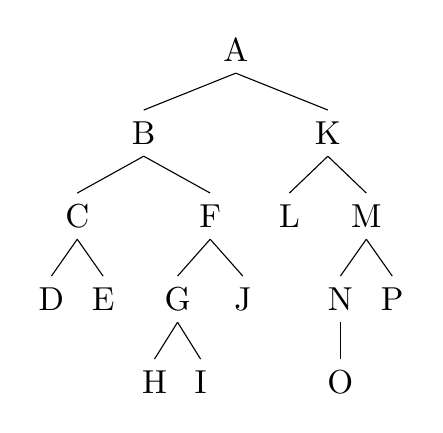
\begin{tikzpicture}
	\tikzset{every tree node/.append style={scale=1.2}}
	\Tree [.A [.B [.C D E ][.F [.G H I ] J ]][.K L [.M [.N O ] P ]]]
\end{tikzpicture}\hfill\null
\par\vspace*{3ex}

\quad\begin{tabular}[t]{r@{\hskip 8pt}p{0.45\linewidth}!{\color{gray!25}\vline}@{\hskip 1.3cm}l}
 1. & List all the nodes c-commanded by K.       & B, C, D, E, F, G, H, I, J \\
 2. & List all the nodes c-commanded by J.       & G, H, I \\
 3. & List all the nodes c-commanded by A.       & $\varnothing$ \\
 4. & List all the nodes c-commanded by D.       & E \\
 5. & List all the nodes c-commanded by P.       & N, O \\
 6. & The node I precedes K here.                & \rtrue{} / \wfalse \\
 7. & The nodes L and F are sisters.             & \wtrue{} / \rfalse \\
 8. & The node L c-commands F.                   & \wtrue{} / \rfalse \\
 9. & The node B c-commands C.                   & \wtrue{} / \rfalse \\
10. & The set \{H, I, J\} is a constituent here. & \rtrue{} / \wfalse
\end{tabular}

\newpage\exercise{Exercise 2: Binding Principles (Carnie, Chapter 5 -- GPS 4)}{12}

Explain why the following sentences are ungrammatical. For each sentence, say what the binding
domain of the NP causing the problem is, whether it is c-commanded by its binder (antecedent), and
name the binding condition that is violated.
\par\vspace*{12pt}
\emph{binding domain}: the clause (TP) containing the NP (anaphor, pronoun, or R-expression)
\begin{enumerate}[label=\alph*)]
	\item *Michael\npi{} loves him\npi.
	\begin{ex2response}{\begin{tabular}[t]{>{\footnotesize\bfseries}rl}
		domain & \emph{Michael loves him}\\
		c-command & \npb{Michael} c-commands \npb{him}\\
		condition & pronoun must be free in its binding domain
	\end{tabular}}
		\tikzset{frontier/.style={distance from root=70pt}}
		\Tree 	[.TP [.NP\npi{} [.N \edge[draw=none]; \qtl{Michael} ]]
			[.VP [.V \edge[draw=none]; \qtl{loves} ]
			[.\textcolor{red}{NP\npi{}}
			[.N \edge[draw=none]; \qtl{\textcolor{red}{him}} ]]]]
	\end{ex2response}

	\item *He\npi{} loves Michael\npi.
	\begin{ex2response}{\begin{tabular}[t]{>{\footnotesize\bfseries}rl}
		domain & \emph{He loves Michael} \\
		c-command & \npb{Michael} does not c-command \npb{he} \\
		condition & binder must c-command bindee \\
		& pronoun must be free in its binding domain
	\end{tabular}}
		\tikzset{frontier/.style={distance from root=70pt}}
		\Tree	[.TP [.\textcolor{red}{NP\npi{}}
			[.N \edge[draw=none]; \qtl{\textcolor{red}{He}} ]]
			[.VP [.V \edge[draw=none]; \qtl{loves} ]
			[.NP\npi{} [.N \edge[draw=none]; \qtl{Michael} ]]]]
	\end{ex2response}

	\item *Michael\npi's father\npi[j] loves himself\npi.
	\begin{ex2response}{\begin{tabular}[t]{>{\footnotesize\bfseries}rl}
		domain & \emph{Michael's father loves himself}\\
		c-command & \npb{Michael} does not c-command \npb{himself}\\
		condition & binder must c-command bindee \\
		& anaphor must be bound in its binding domain
	\end{tabular}}
		\tikzset{frontier/.style={distance from root=70pt}}
		\Tree	[.TP [.NP\npi[j] [.NP\npi{} [.N \edge[draw=none]; \qtl{Michael's} ]]
			[.N \edge[draw=none]; \qtl{father} ]]
			[.VP [.V \edge[draw=none]; \qtl{loves} ]
			[.\textcolor{red}{NP\npi{}}
			[.N \edge[draw=none]; \qtl{\textcolor{red}{himself}} ]]]]
	\end{ex2response}

	\item *Michael\npi's father\npi[j] loves him\npi[j].
	\begin{ex2response}{\begin{tabular}[t]{>{\footnotesize\bfseries}rl}
		domain & \emph{Michael's father loves him}\\
		c-command & \npb{Michael's father} c-commands \npb{him}\\
		condition & pronoun must be free in its binding domain
	\end{tabular}}
		\tikzset{frontier/.style={distance from root=70pt}}
		\Tree	[.TP [.NP\npi[j] [.NP\npi{} [.N \edge[draw=none]; \qtl{Michael's} ]]
			[.N \edge[draw=none]; \qtl{father} ]]
			[.VP [.V \edge[draw=none]; \qtl{loves} ]
			[.\textcolor{red}{NP\npi[j]}
			[.N \edge[draw=none]; \qtl{\textcolor{red}{him}} ]]]]
	\end{ex2response}

	\item *Susan\npi{} thinks that John should marry herself\npi.
	\begin{ex2response}{\begin{tabular}[t]{>{\footnotesize\bfseries}rl}
		domain & \emph{John should marry herself}\\
		c-command & \npb{Susan} c-commands \npb{herself}\\
		condition & anaphor must be bound in its \\
		& \quad binding domain
	\end{tabular}}
		\tikzset{frontier/.style={distance from root=130pt}}
		\Tree	[.TP [.NP\npi{} [.N \edge[draw=none]; \qtl{Susan} ]]
			[.VP [.V \edge[draw=none]; \qtl{thinks} ]
			[.CP [.C \edge[draw=none]; \qtl{that} ]
			[.TP [.NP [.N \edge[draw=none]; \qtl{John} ]]
			[.T \edge[draw=none]; \qtl{should} ]
			[.VP [.V \edge[draw=none]; \qtl{marry} ]
			[.\textcolor{red}{NP\npi}
			[.N \edge[draw=none]; \qtl{\textcolor{red}{herself}} ]]]]]]]
	\end{ex2response}

	\item *John thinks that Susan\npi{} should kiss her\npi.
	\begin{ex2response}{\begin{tabular}[t]{>{\footnotesize\bfseries}rl}
		domain & \emph{Susan should kiss her}\\
		c-command & \npb{Susan} c-commands \npb{her}\\
		condition & pronoun must be free in its \\
		& \quad binding domain
	\end{tabular}}
		\tikzset{frontier/.style={distance from root=130pt}}
		\Tree	[.TP [.NP [.N \edge[draw=none]; \qtl{John} ]]
			[.VP [.V \edge[draw=none]; \qtl{thinks} ]
			[.CP [.C \edge[draw=none]; \qtl{that} ]
			[.TP [.NP\npi{} [.N \edge[draw=none]; \qtl{Susan} ]]
			[.T \edge[draw=none]; \qtl{should} ]
			[.VP [.V \edge[draw=none]; \qtl{kiss} ]
			[.\textcolor{red}{NP\npi}
			[.N \edge[draw=none]; \qtl{\textcolor{red}{her}} ]]]]]]]
	\end{ex2response}
\end{enumerate}

\newpage\exercise{Exercise 3: Binding and Wh-questions (Carnie, Chapter 5 -- CPS 1)}{4}

What problem(s) does the following sentence raise for the binding theory as we have sketched in
this chapter? \textbf{Think of a solution that could explain why this sentence is grammatical. It's
ok to speculate and think of more than one potential explanation.} Hint: consider the non-question
form of this sentence \emph{John despises these pictures of himself.} (Another hint: one possible
solution can relate to one of the possibilities explored in Crain and Nakayama's paper we read).

\begin{enumerate}[label=(\arabic*)]
	\item Which pictures of himself\npi{} does John\npi{} despise?
\end{enumerate}

Assume the following tree for this sentence:
\par\vspace*{3ex}
\hfill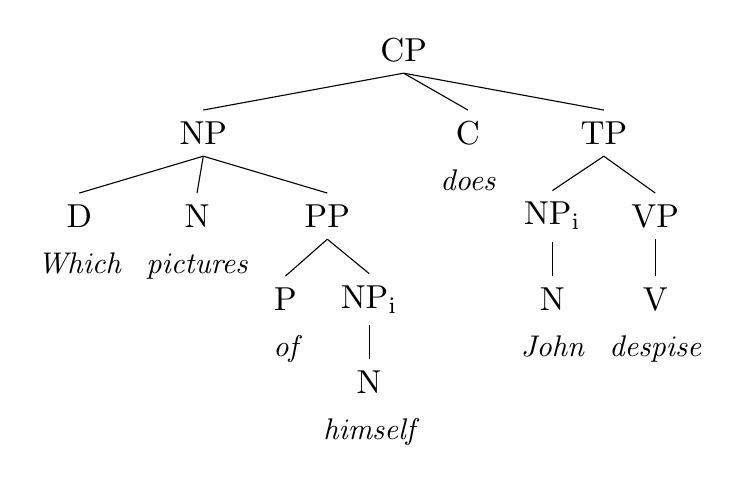
\begin{tikzpicture}
	\tikzset{every tree node/.style={scale=1.2}}
	\tikzset{every leaf node/.style={scale=0.9,font=\itshape}}
	\tikzset{frontier/.style={level distance=18pt}}
	\Tree	[.CP [.NP [.D \edge[draw=none]; \qtl{Which} ]
		[.N \edge[draw=none]; \qtl{pictures} ]
		[.PP [.P \edge[draw=none]; \qtl{of} ]
		[.NP\npi{} [.N \edge[draw=none]; \qtl{himself} ]]]]
		[.C \edge[draw=none]; \qtl{does} ]
		[.TP [.NP\npi{} [.N \edge[draw=none]; \qtl{John} ]]
		[.VP [.V \edge[draw=none]; \qtl{despise} ]]]]
\end{tikzpicture}\hfill\null
\begin{itemize}[noitemsep]
	\item The given tree breaks currently established PS-rules for CPs
	\par\hfill
	\textbf{expected}\quad CP $\rightarrow$ (C) TP\hspace*{1cm}
	\textbf{encountered}\quad CP $\rightarrow$ NP C TP\hfill\null

	\item The given tree contradicts our current defition of \textbf{binding}, which requires
	      the binder to c-command the bindee.

	\item The given tree violates \textbf{Binding Principle A}, which states that an anaphor must be
	      bound in its own binding domain.
\end{itemize}
\hfill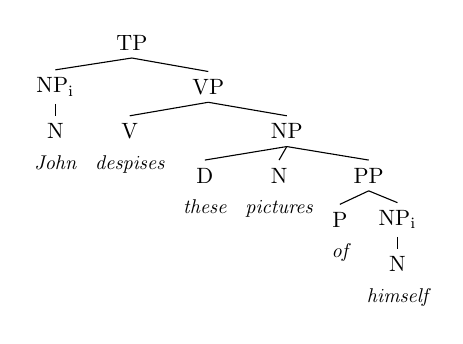
\begin{tikzpicture}
	\tikzset{every tree node/.style={scale=0.8}}
	\tikzset{every leaf node/.style={scale=0.9,font=\itshape}}
	\tikzset{interior/.style={level distance=16pt}}
	\tikzset{frontier/.style={level distance=12pt}}
	\Tree	[.TP [.NP\npi{} [.N \edge[draw=none]; \qtl{John} ]]
		[.VP [.V \edge[draw=none]; \qtl{despises} ]
		[.NP [.D \edge[draw=none]; \qtl{these} ]
		[.N \edge[draw=none]; \qtl{pictures} ]
		[.PP [.P \edge[draw=none]; \qtl{of} ]
		[.NP\npi{} [.N \edge[draw=none]; \qtl{himself} ]]]]]]
\end{tikzpicture}\hfill\null
\par\vspace*{3ex}

After examing the non-question form of the given sentence, I think the only problem with binding
theory that this example reveals is the definition of \textbf{binding domain}. Primarily, I believe
that this is an example of some sort of syntactical restructuring to signify a question unrelated
to binding; maybe \npb{Which pictures of himself} has some sort of dependence relationship to
\emph{[\textsubscript{TP} John despise]}. I think this restructuring may alter the definition of 
not only \textbf{binding domain}, but the definitions of some of the structural relations between
tree nodes as well.

\newpage\exercise{Exercise 4: Complements \& Adjuncts (Carnie, Chapter 6 -- GPS1)}{12}

Using the tests you have been given in chapter 6 (reordering, adjacency, conjunction of likes,
\emph{one}-replacement) determine whether the PPs in the following NPs are complements or adjuncts.
Use at least 3 tests for each PP. Give the examples that you used in constructing your tests. Some
of the NPs have multiple PPs. Be sure to answer the question for every PP in the NP.

\begin{enumerate}[label=\alph*)]
	\item A container [of flour]
	\par\vspace*{0.5ex}
	\begin{minipage}[c]{0.7\textwidth}
		\par\vspace{0.5ex}{\small\bfseries Reordering}
		\begin{enumerate}[label=(\arabic*),nosep]
			\item A container [of flour] [beside the dumpster]
			\item *A container [beside the dumpster] [of flour]
		\end{enumerate}
		{\small\bfseries Conjuction of Likes}
		\begin{enumerate}[label=(\arabic*),nosep]
			\setcounter{enumii}{2}
			\item A container [of souls] and [of flour]
			\item *A container [beside the dumpster] and [of flour]
		\end{enumerate}
		{\small\bfseries \emph{One}-replacement}
		\begin{enumerate}[label=(\arabic*),nosep]
			\setcounter{enumii}{4}
			\item The one of flour
		\end{enumerate}
	\end{minipage}\hfill\begin{minipage}[c]{0.2\textwidth}
		\hfill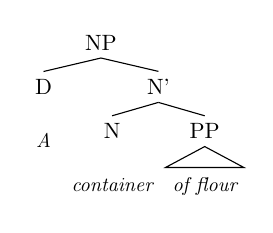
\begin{tikzpicture}
			\tikzset{every tree node/.style={scale=0.8}}
			\tikzset{every leaf node/.style={scale=0.9,font=\itshape}}
			\tikzset{interior/.style={level distance=16pt}}
			\tikzset{frontier/.style={level distance=20pt}}
			\Tree	[.NP [.D \edge[draw=none]; \qtl{A} ]
				[.N' [.N \edge[draw=none]; \qtl{container} ]
				[.PP \edge[roof]; \qtl{of flour} ]]]
		\end{tikzpicture}
	\end{minipage}

	\par\vspace*{2ex}
	I believe that (5) can be grammatical, but many do not. \ppb{of flour} can be neither
	reordered nor conjoined with known adjunct \ppb{beside the dumpster}. Thus, \ppb{of flour}
	is a complement.
	\par\vspace*{2ex}

	\item A container [with a glass lid]
	\par\vspace*{0.5ex}
	\begin{minipage}[c]{0.65\textwidth}
		\par\vspace{0.5ex}{\small\bfseries Reordering}
		\begin{enumerate}[label=(\arabic*),nosep]
			\item A container [with a glass lid] [abaft the deckhouse]
			\item A container [abaft the deckhouse] [with a glass lid]
		\end{enumerate}
		{\small\bfseries Conjuction of Likes}
		\begin{enumerate}[label=(\arabic*),nosep]
			\setcounter{enumii}{2}
			\item *A container [with a glass lid] and [of heroin]
			\item A container [with a glass lid] and [betwixt those junkies]
		\end{enumerate}
		{\small\bfseries \emph{One}-replacement}
		\begin{enumerate}[label=(\arabic*),nosep]
			\setcounter{enumii}{4}
			\item The one with a glass lid
		\end{enumerate}
	\end{minipage}\hfill\begin{minipage}[c]{0.25\textwidth}
		\hfill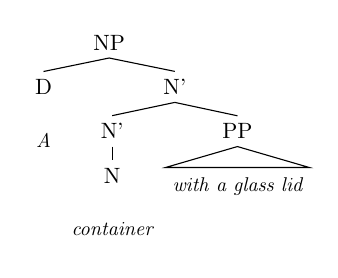
\begin{tikzpicture}
			\tikzset{every tree node/.style={scale=0.8}}
			\tikzset{every leaf node/.style={scale=0.9,font=\itshape}}
			\tikzset{interior/.style={level distance=16pt}}
			\tikzset{frontier/.style={level distance=20pt}}
			\Tree [.NP
				[.D \edge[draw=none]; \qtl{A} ]
				[.N' [.N' [.N \edge[draw=none]; \qtl{container} ]]
					[.PP \edge[roof]; \qtl{with a glass lid} ]]]
		\end{tikzpicture}
	\end{minipage}

	\par\vspace*{2ex}
	\ppb{with a glass lid} can be reordered with other PPs, can be conjoined with adjuncts but
	not complements, and can stand next to the word \emph{one}; it is an adjunct.
	\par\vspace*{2ex}

	\item The collection [of figurines] [in the window]
	\par\vspace*{0.5ex}
	\begin{minipage}[c]{0.58\textwidth}
		\par\vspace{0.5ex}{\small\bfseries Reordering}
		\begin{enumerate}[label=(\arabic*),nosep]
			\item *The collection [in the window] [of figurines]
			\item The collection [in the window] [along the sill]
		\end{enumerate}
		{\small\bfseries Conjuction of Likes}
		\begin{enumerate}[label=(\arabic*),nosep]
			\setcounter{enumii}{2}
			\item *The collection [of figurines] and [in the window]
			\item The collection [of figurines] and [of marsupials]
			\item The collection [under the bed] and [in the window]
		\end{enumerate}
		{\small\bfseries \emph{One}-replacement}
		\begin{enumerate}[label=(\arabic*),nosep]
			\setcounter{enumii}{5}
			\item The one [in the window]
			\item *The one [of figurines] [in the window]
		\end{enumerate}
	\end{minipage}\hfill\begin{minipage}[c]{0.32\textwidth}
		\hfill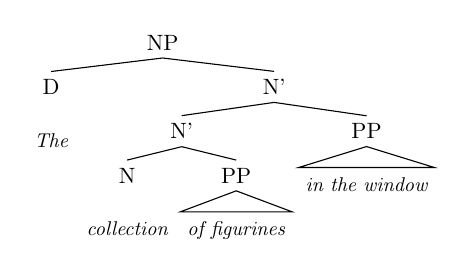
\begin{tikzpicture}
			\tikzset{every tree node/.style={scale=0.8}}
			\tikzset{every leaf node/.style={scale=0.9,font=\itshape}}
			\tikzset{interior/.style={level distance=16pt}}
			\tikzset{frontier/.style={level distance=20pt}}
			\Tree [.NP
				[.D \edge[draw=none]; \qtl{The} ]
				[.N' [.N' [.N \edge[draw=none]; \qtl{collection} ]
				[.PP \edge[roof]; \qtl{of figurines} ]]
				[.PP \edge[roof]; \qtl{in the window} ]]]
		\end{tikzpicture}
	\end{minipage}

	\par\vspace*{2ex}
	\ppb{of figurines} is a complement: it cannot be reordered (1), it can be combined with
	other complements (4) but not adjuncts (3), and it cannot stand by \emph{one} (7). Examples
	(2), (3), (5), and (6) show that \ppb{in the window} is an adjunct.
\end{enumerate}

\newpage\exercise{Exercise 5: X'-theory (from Carnie, Chapter 6 -- GPS 7)}{39}
Draw the X-bar-theoretic trees for the following sentences.

\begin{enumerate}[label=\alph*)]
	\item Abelard wrote a volume of poems in Latin for Héloïse.
	\begin{ex5response}
		\Tree	[.TP [.NP [.N' [.N \edge[draw=none]; \qtl{Abelard} ]]]
			[.VP [.V' [.V' [.V \edge[draw=none]; \qtl{wrote} ]
			[.NP [.D \edge[draw=none]; \qtl{a} ]
			[.N' [.N' [.N \edge[draw=none]; \qtl{volume} ]
			[.PP [.P' [.P \edge[draw=none]; \qtl{of} ]
			[.NP [.N' [.N \edge[draw=none]; \qtl{poems} ]]]]]]
			[.PP [.P' [.P \edge[draw=none]; \qtl{in} ]
			[.NP [.N' [.N \edge[draw=none]; \qtl{Latin} ]]]]]]]]
			[.PP [.P' [.P \edge[draw=none]; \qtl{for} ]
			[.NP [.N' [.N \edge[draw=none]; \qtl{Héloïse} ]]]]]]]]
	\end{ex5response}
	In addition to the position shown in the tree as an adjunct of \npb{a volume of poems},
	\ppb{in Latin} can be an adjunct of either \npb{poems} or \emph{[\textsubscript{VP} wrote a
	volume of poems for Héloïse]}.

	\item Armadillos from New York often destroy old pillowcases with their snouts.
	\begin{ex5response}
		\Tree 	[.TP [.NP [.N' [.N' [.N \edge[draw=none]; \qtl{Armadillos} ]]
			[.PP [.P' [.P \edge[draw=none]; \qtl{from} ]
			[.NP [.N' [.N \edge[draw=none]; \qtl{New York} ]]]]]]]
			[.VP [.V' [.V' [.AdvP [.Adv' [.Adv \edge[draw=none]; \qtl{often} ]]]
			[.V' [.V \edge[draw=none]; \qtl{destroy} ] [.NP [.N'
			[.AdjP [.Adj' [.Adj \edge[draw=none]; \qtl{old} ]]]
			[.N' [.N \edge[draw=none]; \qtl{pillowcases} ]]]]]]
			[.PP [.P' [.P \edge[draw=none]; \qtl{with} ]
			[.NP [.D \edge[draw=none]; \qtl{their} ]
			[.N' [.N \edge[draw=none]; \qtl{snouts} ]]]]]]]]
	\end{ex5response}

	\item People with boxes of old clothes lined up behind the door of the building with the
	      leaky roof.
	\begin{ex5response}
		\tikzset{sibling distance=-1.8pt}
		\Tree	[.TP [.NP [.N' [.N' [.N \edge[draw=none]; \qtl{People} ]]
			[.PP [.P' [.P \edge[draw=none]; \qtl{with} ]
			[.NP [.N' [.N \edge[draw=none]; \qtl{boxes} ]
			[.PP [.P' [.P \edge[draw=none]; \qtl{of} ]
			[.NP [.N' [.AdjP [.Adj' [.Adj \edge[draw=none]; \qtl{old} ]]]
			[.N' [.N \edge[draw=none]; \qtl{clothes} ]]]]]]]]]]]]
			[.VP [.V' [.V' [.V \edge[draw=none]; \qtl{lined up} ]]
			[.PP [.P' [.P \edge[draw=none]; \qtl{behind} ]
			[.NP [.D \edge[draw=none]; \qtl{the} ]
			[.N' [.N \edge[draw=none]; \qtl{door} ]
			[.PP [.P' [.P \edge[draw=none]; \qtl{of} ]
			[.NP [.D \edge[draw=none]; \qtl{the} ]
			[.N' [.N' [.N \edge[draw=none]; \qtl{building} ]]
			[.PP [.P' [.P \edge[draw=none]; \qtl{with} ]
			[.NP [.D \edge[draw=none]; \qtl{the} ]
			[.N' [.AdjP [.Adj' [.Adj \edge[draw=none]; \qtl{leaky} ]]]
			[.N' [.N \edge[draw=none]; \qtl{roof} ]]]]]]]]]]]]]]]]]
	\end{ex5response}

	\item My favorite language is a language with simple morphology and complicated syntax.
	\begin{ex5response}
		\Tree	[.TP [.NP [.D \edge[draw=none]; \qtl{My} ]
			[.N' [.AdjP [.Adj' [.Adj \edge[draw=none]; \qtl{favorite} ]]]
			[.N' [.N \edge[draw=none]; \qtl{language} ]]]]
			[.VP [.V' [.V \edge[draw=none]; \qtl{is} ]
			[.NP [.D \edge[draw=none]; \qtl{a} ]
			[.N' [.N' [.N \edge[draw=none]; \qtl{language} ]]
			[.PP [.P' [.P \edge[draw=none]; \qtl{with} ]
			[.NP [.N' [.N' [.AdjP [.Adj' [.Adj \edge[draw=none]; \qtl{simple} ]]]
			[.N' [.N \edge[draw=none]; \qtl{morphology} ]]]
			[.Conj \edge[draw=none]; \qtl{and} ]
			[.N' [.AdjP [.Adj' [.Adj \edge[draw=none]; \qtl{complicated} ]]]
			[.N' [.N \edge[draw=none]; \qtl{syntax} ]]]]]]]]]]]]
	\end{ex5response}

	\item The collection of syntax articles with the red cover bores students of syntax in
	      Tucson.
	\begin{ex5response}
		\tikzset{sibling distance=0pt}
		\Tree [.TP [.NP [.D \edge[draw=none]; \qtl{The} ]
			[.N' [.N' [.N \edge[draw=none]; \qtl{collection} ]
			[.PP [.P' [.P \edge[draw=none]; \qtl{of} ]
			[.NP [.N' [.AdjP [.Adj' [.Adj \edge[draw=none]; \qtl{syntax} ]]]
			[.N' [.N \edge[draw=none]; \qtl{articles} ]]]]]]]
			[.PP [.P' [.P \edge[draw=none]; \qtl{with} ]
			[.NP [.D \edge[draw=none]; \qtl{the} ]
			[.N' [.AdjP [.Adj' [.Adj \edge[draw=none]; \qtl{red} ]]]
			[.N' [.N \edge[draw=none]; \qtl{cover} ]]]]]]]]
			[.VP [.V' [.V \edge[draw=none]; \qtl{bores} ]
			[.NP [.N' [.N' [.N \edge[draw=none]; \qtl{students} ]
			[.PP [.P' [.P \edge[draw=none]; \qtl{of} ]
			[.NP [.N' [.N \edge[draw=none]; \qtl{syntax} ]]]]]]
			[.PP [.P' [.P \edge[draw=none]; \qtl{in} ]
			[.NP [.N' [.N \edge[draw=none]; \qtl{Tuscon} ]]]]]]]]]]
	\end{ex5response}
\end{enumerate}
\end{document}
